
\subsubsection{Notificacions}
\label{sec:patro_notificacio}

El patró Notificacions permet la comunicació entre objectes sense implicar que aquests estiguin acoblats. Un objecte pot enviar informació a els altres objectes sense informació especifica d'aquests objectes. Els objectes que estan interessats en rebre alguna informació es registren utilitzant una instància de de la classe NSNotificationCenter\footnote{Centre de notificacions de la llibreria d'\textit{Apple}}. S'anomenen observadors els objectes registrats, és per això que sovint aquest patró de disseny també és anomenat patró Observador.

Quan s'envia una notificació al centre de notificacions, aquest distribueix la notificació a tots els observadors que s'han registrat a aquell tipus de notificació. 

\begin{figure}[ht]
    \centering
    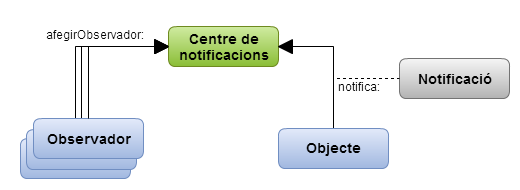
\includegraphics[scale=1]{Memoria/Arquitectura/iOS/patro-notificacio.png}
    \caption{Comunicació entre el centre de notificacions i els observadors.}
    \label{fig:patro_notificacio}
\end{figure}


L'objecte que envia un missatge cap al centre de notificacions no necessita conèixer quins observadors existeixen ni quants hi han. De manera similar, els observadors no necessiten conèixer l'origen de les notificacions rebudes. A la figura \ref{fig:patro_notificacio} es mostra la comunicació entre el centre de notificacions i els observadors, així com la comunicació amb l'objecte que envia la notificació.


